\documentclass{bioinfo}
\copyrightyear{2014}
\pubyear{2014}
\usepackage{amssymb}
\usepackage{algorithm}
\usepackage{algpseudocode}

\begin{document}
\firstpage{1}

\title[Sequence clustering by all pairs-search]{Starcode: sequence
clustering based on all-pairs search }
\author[Valera Zorita \textit{et~al}.]{Eduard Valera Zorita\,$^{1,2}$, Pol
Cusc\'o\,$^{1,2}$ and Guillaume Filion\,$^{1,2}$\footnote{to whom
correspondence should be addressed}}
\address{$^{1}$Genome Architecture, Gene Regulation, Stem Cells and
Cancer Programme, Centre for Genomic Regulation (CRG), Dr. Aiguader 88,
08003 Barcelona, Spain.\\
$^{2}$Universitat Pompeu Fabra (UPF), Barcelona, Spain.}

\history{Received on XXXXX; revised on XXXXX; accepted on XXXXX}

\editor{Associate Editor: XXXXXXX}

\maketitle

\begin{abstract}
\section{Motivation:}
The increasing throughput of sequencing technologies offers new
applications and challenges for computational biology. In many
of those applications, sequencing errors need to be corrected.
This is particularly important when sequencing reads from an
unknwon reference such as random DNA barcodes.
In this case, error correction can be
done by performing a pairwise comparison of all the barcodes,
which is computationally complex problem.

\section{Results:}
Here we address this challenge and describe an exact algorithm to
determine which pairs of sequences lie within a given Levenshtein
distance. For error correction or redundancy reduction purposes,
matched pairs are then merged into clusters of similar sequences.
The effiency of starcode is attributable to
the poucet search, a novel implementation of the Needleman-Wunsch
algorithm performed on the nodes of a trie. On the task of matching
random barcodes, starcode outperforms sequence clustering algorithms
in both speed and precision.

\section{Availability and implementation:}
The C source code is available at http://github.com/gui11aume/starcode.

\section{Contact:} \href{guillaume.filion@gmail.com}{guillaume.filion@gmail.com}
\end{abstract}


\section{Introduction}

All sequencing technologies have a certain degree of imprecision.
For instance, the Illumina platform \citep{pmid16056220} has a 1-2\%
error rate consisting of substitutions \citep{pmid18660515, pmid21576222}
and the PacBio platform has a 15\% error rate consisting of insertions
and deletions \citep{pmid19023044}. The enormous throughput of such
technologies has recently created additional needs for developing
efficient error correction algorithms.

Sequencing errors can be discovered by comparing the reads to a
reference genome. However, such a reference is not always available.
When the sequences are random or taken from an unknown source,
clustering is the main strategy to correct the errors.
For instance, this situation arises when using random barcodes to
track cells or transcripts \citep{pmid18809713, pmid23953119}.
Sequencing errors will create erroneous (nonexistent) barcodes
that have to be removed.

Sequence clustering can be viewed as a community detection problem
on graphs, where nodes represent sequences and edges represent matches
between related sequences. The process consists of a matching phase
(the most computationally intensive), where the graph is constructed,
and a clustering phase where communities are identified.

Here we describe a sequence clustering algorithm called ``starcode''
in reference to clusters of random barcodes, which typically have a star
shape.  Starcode is based on all-pairs search, \textit{i.e.} all the pairs
of sequences below a given Levenshtein distance are identified during
the graph construction phase. Matching is carried out by lossless
filtration, followed by an exhaustive search on the branches of a
prefix trie.  The novelty of the algorithm is the poucet strategy,
which uses the redundancy of alphabetically sorted sequences to avoid
unnecessary recomputations and gain speed. 

In this article we present and benchmark starcode. We show that on
real biological datasets, starcode is orders of magnitude faster than
existing sequence clustering software. Even though starcode was
designed for error correction, we also show that it can be used for
other problems. As an illustration, we use it to identify enriched
motifs in a bacterial genome and in protein-RNA interaction
experiments.

\begin{methods}
\section{Methods}
\subsection{Inexact string matching using tries}
The matching method of starcode is based on a variation of the
Needleman-Wunsch (NW) algorithm \citep{pmid5420325}. In the
original algorithm (Figure \ref{fig:NW}a), the Levenshtein
distance between two sequences is found by applying a recurrence
relation throughout a matrix of $mn$ terms (the edit matrix),
where $m$ and $n$ are the respective sequence lengths. The complexity
of this dynamic programming approach is $O(mn)$. 

\begin{figure}[!tpb]
\centerline{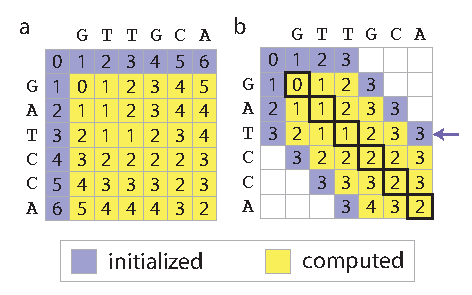
\includegraphics{NW.pdf}}
\caption{Needleman-Wunsch (NW) sequence comparison. \textbf{a}
Comparison of GTTGCA and GATCCA. The margins of the edit matrix
(purple) are initialized and the cells (yellow)
are computed from left to right and from top to bottom by the NW
dynamic programming algorithm. $E[i,j]$, the term of
coordinates $(i,j)$ is computed as
$\min(E[i-1,j]+1, E[i,j-1]+1, E[i-1,j-1]+\Delta(i,j))$, where
$\Delta(i,j) = 0$ if the $i$-th symbol from the first sequence is the
same as the $j$-th symbol from the second, and $\Delta(i,j) = 1$
otherwise. The Levenshtein distance between the two sequences is the
value of the bottom right cell. \textbf{b} Lower complexity algorithm
to determine whether GTTGCA and GATCCA are 2-matches.
The values in the purple cells are set
during initialization. The dynamic programming algorithm proceeds as
above, with the difference that it is aborted if the value of a
diagonal cell (bold borders) is larger than 2. The values in the
purple cells may differ from the original NW scheme (purple arrow),
but the values in the yellow cells are nevertheless identical.
The values of the white cells are never computed, which contributes to
reducing the complexity.}\label{fig:NW}
\end{figure}

In many instances, the information of interest is to find out
whether the sequences are $\tau$-matches (\textit{i.e.} their distance
is less then or equal to a fixed threshold $\tau$).
In that case, the complexity can be reduced to $O(\tau \min(m,n))$.
Instead of computing all the terms of the edit matrix, it is initialized
as shown on Figure \ref{fig:NW}b and only the terms around the diagonal
are computed. If a diagonal term has a value greater than $\tau$,
the process is halted because the sequences are not $\tau$-matches.

This method can be used to match sequences against a prefix tree,
also known as a trie \citep{ukkonen}. The terms of the edit matrix
are updated row-wise while a depth-first search traverses the trie
(Figure \ref{fig:trie}). Every time a node is visited,
a row is computed, and every time the search backtracks, a row is
erased. If the threshold value $\tau$
is exceeded for a diagonal term, the Levenshtein distance for all the
downstream sequences is also necessarily greater than $\tau$. Therefore,
no more hits are to be discovered in this path and the depth-first
search backtracks to the parent node. When the process halts, every
tail node (corresponding to a sequence of the database) on the path
of this search is a $\tau$-match of the query. This method is
efficient because it eliminates large areas of the search space, and
because the NW comparison of the query with each prefix of the database
is computed only once.

\begin{figure}[!tpb]
\centerline{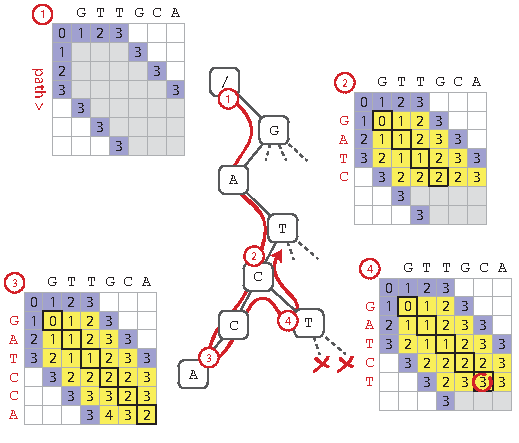
\includegraphics{trie.pdf}}
\caption{NW algorithm on tries. Each sequence of the index is a
path in the trie. The query GTTGCA is written at the top of the matrix,
which is initialized as shown on Figure \ref{fig:NW}b. The trie is
traversed by a depth-first search (red path). At each
depth, the node added to the path is written on the left of the edit
matrix and the row is computed. Checkpoints from 1 to 4 (circled red
numbers) show the state of the edit matrix as the search proceeds. The
node labeled 3 is a leaf and thus corresponds to a 2-match of the
query. After discovering the hit, the search path backtracks to the
node labeled 2 and the last rows of the edit matrix are erased.
The search path then goes to the node labeled 4, in which case the
newly computed diagonal cell exceeds the threshold (circled in red).
Even if this node has children, they are not visited (red crosses)
because there is no 2-match to discover.}
\label{fig:trie}
\end{figure}


\subsection{The poucet search algorithm}
The search strategy can be further improved. If two consecutive
queries share a prefix of length $k$, the succession of computations
up to the $k$-th row of the edit matrix will be exactly the same
for both queries. Therefore, computation intermediates can be
stored in the nodes of the trie, so that the next trie search can start
at depth $k$. However, storing the rows of the edit matrix in the nodes
meets some difficulty. Indeed, on the $k$-th row, the terms on the
right side of the diagonal depend on characters that are not shared
between the two queries. This issue is solved by storing in each
node a combination of row and column terms that form an angle shape,
looking like a horizontally flipped L (Figure \ref{fig:poucet}).
Using this structure, the computation intermediates stored in a
node at depth $k$ depend only on the first $k$ characters of the
query.

To take full advantage of this property, the input sequences are
sorted alphabetically, which maximize prefix sharing between
consecutive queries. In the fairy tale ``Le Petit Poucet'', the
hero seeds white pebbles for his older brothers to find their way
home, which is reminiscent of the way a smaller query (in alphabetical
order) paves the way for the next. We therefore called this search
algorithm ``poucet''.

\begin{figure}[!tpb]
\centerline{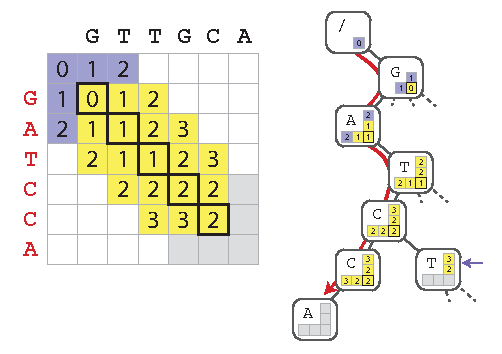
\includegraphics{poucet.pdf}}
\caption{Poucet search algorithm. The algorithm proceeds with the
same principles as shown on Figure \ref{fig:trie} with the difference
that the edit matrix is not updated row-wise, but along a horizontally
flipped L. As the depth-first search proceeds, these values
are stored in the nodes of the trie. Since the values in the vertical
part of the flipped L are the same for every child of a node,
they are computed only once (purple arrow). The values in the grey
cells will be computed as the search path (red) visits the node.
Storing the intermediates in the nodes allows the next query to
restart at depth $k$ if it shares a common prefix of length
$k$ with the current query.}
\label{fig:poucet}
\end{figure}


\subsection{Lossless filtration}
When a query has no match, it is advantageous to omit the trie
search. To this end, starcode uses a partition
approach similar to that described by \cite{WuManber1992}. The query
is initially partitioned in $\tau+1$ segments. Assuming that all the
segments have length at least $\tau$, then every $\tau$-match present
in the database will contain at least a verbatim copy of one of the
query segments. Indeed, there are at most $\tau$ editions between
the query and the match to be distributed in $\tau+1$ regions, so at
least one segment is unmodified. Due to potential insertions and
deletions in the preceding segments, the shared segment may be shifted
up to $\tau$ nucleotides on the left (all insertions) or on the right
(all deletions) from its original position in the query.

These observations are the basis of a filtration method with 100\%
specificity. More precisely, the segments are defined as follows:
the first $\tau$ nucleotides of the sequence are removed, and the rest
of the sequence is partitioned in $\tau+1$ segments of sizes differing
by at most 1 (the longer segments always in 3' for consistency). Every
time a sequence is added to the trie, it is partitioned and its
segments are added to $\tau+1$ different indexes. The first fragments
are added to the first index, the second fragments to the second index,
\textit{etc}. Before the search, the query is partitioned in the same
way and its segments are looked up in the indexes. In case no match is
found, this query has no $\tau$-match in the current database,
therefore the trie search is omitted. Conversely, if at least one
segment is found, the trie search must performed.

As mentioned above, segments shared between the query and a
$\tau$-match may be found shifted up to $\tau$ nucleotides. For this
reason, shifted segments of the query are looked up in the indexes
according to the scheme of Figure \ref{fig:filtration}, which ensures
that no match can be missed: the rightmost segment is looked up in the
$\tau$+1-th index, the second rightmost segment and the contiguous
segments shifted by 1 nucleotides are are looked up in the $\tau$-th
index and so on, until the first segment and its contiguous segments
shifted by up to $\tau$ nucleotides are looked up in the first index.

\begin{figure}[!tpb]
\centerline{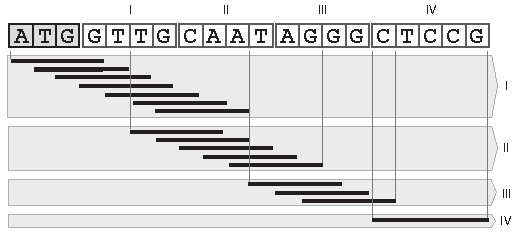
\includegraphics{filtration.pdf}}
\caption{Lossless filtration illustrated by an example sequence
of length 20 with $\tau=3$. The last $\tau$ nucleotides of the query
are removed, and the rest is divided into 4 series of contiguous
segments.  Each series is queried against a different index numbered
I to IV.  For instance, the only segment queried against index I
is GTTG, while those queried against index II are GCAA, CAAT and AATA.
If any of the segments is found in the appropriate index, the trie
search is performed, otherwise it is omited as there can be no
$\tau$-match. Regardless of the result, segments labelled I to IV
are then added to the corresponding respective index (\textit{i.e.}
only one segment is added to each index).}
\label{fig:filtration}
\end{figure}

\subsection{Seek and construct}
To reduce the size of the search space, starcode uses a dynamic
``seek and construct'' approach whereby queries are processed
meanwhile the trie is built. In other words, each sequence is
matched against the trie before it is inserted. If A and B are
mutual $\tau$-matches, either A will be queried when B is in
in the trie, or the converse. Either way, the match A-B is
discovered. This guarantees that every $\tau$-match is discovered,
while maintaining the trie as ``thin'' as possible, thereby reducing
the search time.  The whole matching process is summarized in
the pseudocode shown in Algorithms~\ref{alg:starcode} and
\ref{alg:poucet}.

\begin{algorithm}
  \caption{Starcode algorithm}
  \label{alg:starcode}
  \begin{algorithmic}[1]
    \State \textbf{Define:} $\tau$
    \State \textbf{Variables:} $seed$, $start = 0$,
    $height$, $seq$, $trie$, $lastseq$, $k$
    \State \textbf{Containers:} $hits$, $pebbles$
    \State \textsc{read} sequence file
    \State $height \gets$ \textsc{determine} maximum sequence length
    \State \textsc{pad} sequences up to $height$
    \State \textsc{sort} sequences alphabetically
    \State $k \gets$ \textsc{compute} filter segment lengths
    \State $trie \gets$ \textsc{create} an empty trie of height $height$
    \State \textsc{insert} root node of $trie$ in $pebbles$ at depth 0
    \ForAll{sequences}
    \State $seq \gets$ \textsc{get} next sequence
    \If{at least one $k$-mer of $seq$ is in the filter index}
    \State $seed \gets$ \textsc{length} of shared prefix
    between current and next sequence
    \State $start \gets$ \textsc{length} of shared prefix
    between $seq$ and $lastseq$
    \State \textsc{clear} hits
    \State \textsc{clear} $pebbles$ at depth $>start$
    \ForAll{$pebbles$ at depth $start$}
    \State $node \gets$ \textsc{get} next node from $pebbles$
    \State \textbf{call} \textsc{poucet}($seq$, $node$, $seed$,
    $hits$, $pebbles$)
    \EndFor
    \State \textsc{process} $hits$ and \textsc{link} matches to $seq$
    \State $lastseq \gets seq$
    \EndIf
    \State \textsc{insert} $seq$ path in $trie$
    \State \textsc{insert} $seq$ $k$-mers into the filter index
    \EndFor
  \end{algorithmic}
\end{algorithm}

\begin{algorithm}
  \caption{Poucet search algorithm}
  \label{alg:poucet}
  \begin{algorithmic}[1]
    \Procedure{poucet}{$query$, $node$, $seed$, $hits$, $pebbles$}:
    \State \textsc{compute} $node$-specific column following NW
        \Comment{Fig.1}
    \ForAll{$child$ nodes in $node$}
    \State \textsc{compute} $child$-specific row following NW
        \Comment{Fig.1}
    \State \textsc{compute} center value using row and column
        \Comment{Fig.1}
    \If{center value $>\tau$} \Comment{Mismatches exceeded.}
    \State \textbf{continue} with next $child$
    \EndIf
    \If{$node$ depth = $height$} \Comment{Hit found.}
    \State \textsc{save} $node$ sequence in $hits$
    \State \textbf{continue} with next $child$
    \EndIf
    \If{$node$ depth $\leq seed$}
    \State \textsc{save} $node$ in $pebbles$ at current depth
    \EndIf
    \State \textbf{call} poucet($query$, $child$, $seed$, $hits$, $pebbles$)
    \EndFor
    \EndProcedure
  \end{algorithmic}
\end{algorithm}


\subsection{Parallelization}
Queries are sorted and partitioned in contiguous blocks.
The matching step then proceeds in two phases. In the build phase, a
distinct trie is built from the sequences of each block according
to the algorithm described above. In the second, all the sequence
blocks are queried against all the other tries. If the queries are
partitioned in $N$ blocks, the first phase consists of $N$ seek and
construct jobs, wile the second consists of $N(N-1)/2$ query jobs. In
each phase, the jobs show no dependency on each other, so the
matching algorithm can be efficiently parallelized provided $N$ is
larger than the number of independent threads.

\subsection{Clustering}
The default clustering algorithm of starcode is designed to correct
sequencing error. This method uses message passing \citep{mackay}
to identify and count ``canonical'' sequences (also referred to as
centroids in the clustering terminology). By default, each sequence transfers its
read count to its closest $\tau$-match provided the latter has at least 5
times more counts. If the condition is not met, the transfer does
not take place. If the sequence has several equally close
$\tau$-matches, the counts are split equally among them. The
process is repeated recursively, starting from sequences with
lowest read count. The sequences with a positive read count at
the end of the process are considered canonical. Clusters consist
of all the sequences transferring their read counts to the same
canonical sequence (sequence transferring their read counts to
different canonicals are discarded). Note that the radius of the
clusters can be higher than the maximum distance used for matching.

Since no sequencing technology has an error rate higher than 20\%,
it is expected that sequences appearing from sequencing errors will
always have 5 times or lower read count than the canonical sequence.
Otherwise, sequences are more likely unrelated, or both are derived
from the same canonical sequence. This behavior can be modified with
the command-line option \emph{cluster-ratio} to allow for a more
flexible or more strict clustering, e.g. to cluster unique input
sequences together, \emph{cluster-ratio} must be set to 1.

For other sequence clustering problems, starcode implements a
multi-purpose algorithm called ``sphere clustering''.
In sphere clustering, sequences are sorted by
frequency of occurrence. Starting from the most
frequent, each sequence becomes canonical and claims all its
$\tau$-matches, which forms a cluster of radius $\tau$ (hence the
name). Claimed sequences are immediately removed, so that they can
belong to only one cluster.

\subsection{Benchmark conditions}
All the tests were performed on a 16-core dual-processor
Intel Xeon E5-2687W v2 system with 256~GB of DDR3-RAM at
1866~Mhz. Command-line parameters were set equivalently in all
softwares to run in single-core mode allowing up to 3 mismatches for
input sequences of length 50. Tables \ref{tab:params1} and
\ref{tab:params2} summarize the execution options used in simulation
and real data sets, respectively.

\begin{table}[h]
\centering
\caption{Software execution options used in simulation benchmark.}
%\resizebox{\columnwidth}{!}{
\begin{tabular}{l|l}
    \bf{software} & \bf{command-line options}\\
    \hline
    starcode-1.0 & \texttt{starcode -d3}\\
    slidesort-2 & \texttt{slidesort\_v2 -d 3 -t E -c DNA}\\
    cd-hit-est-4.6.1 & \texttt{cd-hit-est -n 9 -c 0.9 -M 0 -r 0}\\
    seed-1.4.1 & \texttt{SEED --mismatch 3}\\
\end{tabular}
%}
\label{tab:params1}
\end{table}

\begin{table}[h]
\centering
\caption{Software execution options used in real data benchmark.}
%\resizebox{\columnwidth}{!}{
\begin{tabular}{l|l}
    \bf{software} & \bf{command-line options}\\
    \hline
    starcode-1.0 & \texttt{starcode -d3}\\ 
    slidesort-2 & \texttt{slidesort\_v2 -d 3 -u -t E -c DNA}\\
    cd-hit-est-4.6.1 & \texttt{cd-hit-est -n 8 -c 0.94 -M 0}\\
    seed-1.4.1 & \texttt{SEED --mismatch 3 --shift 3}\\ 
    rainbow-2.0.3 & \texttt{rainbow cluster -m 3}
\end{tabular}
%}
\label{tab:params2}
\end{table}


\end{methods}

\section{Results}

\subsection{Presentation and basic performance}
\label{section:performance}
Starcode is a general purpose DNA sequence clustering tool with a
strong focus on error correction. Errors are assumed to be mismatches,
insertions or deletions (the implementation presented here matches
sequences with up to 8 errors). The input sequences can be single
or paired-end reads, with an upper limit of 1024 nucleotides (512
for paired-end). Sequences may be of variable length, they may
be trimmed and filtered for quality or not. File formats compatible
with starcode are raw sequence, raw sequence with count, FASTA or
FASTQ (in which case starcode ignores the quality). Starcode either
returns detailed information of the clustering results, i.e. canonical
sequences, cluster sizes and the complete list of their constituent
sequences. Alternatively, only the canonical sequences are
printed, which is useful to filter out redundant
sequences from input files. By default, clustering is performed under
the assumption that divergence occurs from experimental errors
(sequencing errors, PCR mutations \textit{etc}.) and a more general
algorithm is also available for other clustering problems (an example
of which is given in section \ref{section:motifs}).

We show the basic performance and scalability of starcode on a
dataset of pseudorandom sequences (Figure \ref{fig:perf}). The standard
configuration is a set of 1,000,000 sequences of length 40, running
on 1 thread and with a maximum Levenshtein distance of 3. In each
test, only one parameter is modified while the others are kept
constant. Since the clustering step does not require additional memory
allocation and is significantly faster than all-pairs search, the
performance results presented in Sections \ref{section:performance} and
\ref{section:benchmark} apply for both message-passing and spheres
clustering algorithms.

Figure \ref{fig:perf}a shows the running time of starcode as a
function of the number of input sequences $n$. In double logarithmic
scale the trend is a straight line with slope 1.5, suggesting that the
running time complexity of starcode is lower than quadratic (the
naive implementation of all-pairs search). Note that the sequences of
this dataset have no match, see section \ref{section:benchmark} for
an evaluation of the performance on more realistic datasets.
Figure \ref{fig:perf}b shows that the running time grows exponentially
as a function of the maximum Levenshtein distance used for clustering.
The reason is that the trie fans out exponentially and the search bails
out at a greater depth as the maximum distance increases.
As a function of the sequence length, the running time first increases 
but then plummets and stays low (Figure \ref{fig:perf}c). Beyond a
threshold length, the filtering algorithm starts to be efficient, and
most of the queries are resolved without searching the trie.
Finally, we show the scalability of starcode with increasing number
of threads in Figure \ref{fig:perf}d. The search algorithm is fully
parallel and the relative performance increases linearly up to 12 threads.
The bending observed thereafter has two sources; the first is 
that the input reading and clustering steps are brief but not parallel,
the second is due to hardware limitations, i.e. there is insufficient
memory bandwidth to satisfy the increased demand of parallel memory accesses.

\begin{figure}[!tpb]
% Basic performance figure.
\centerline{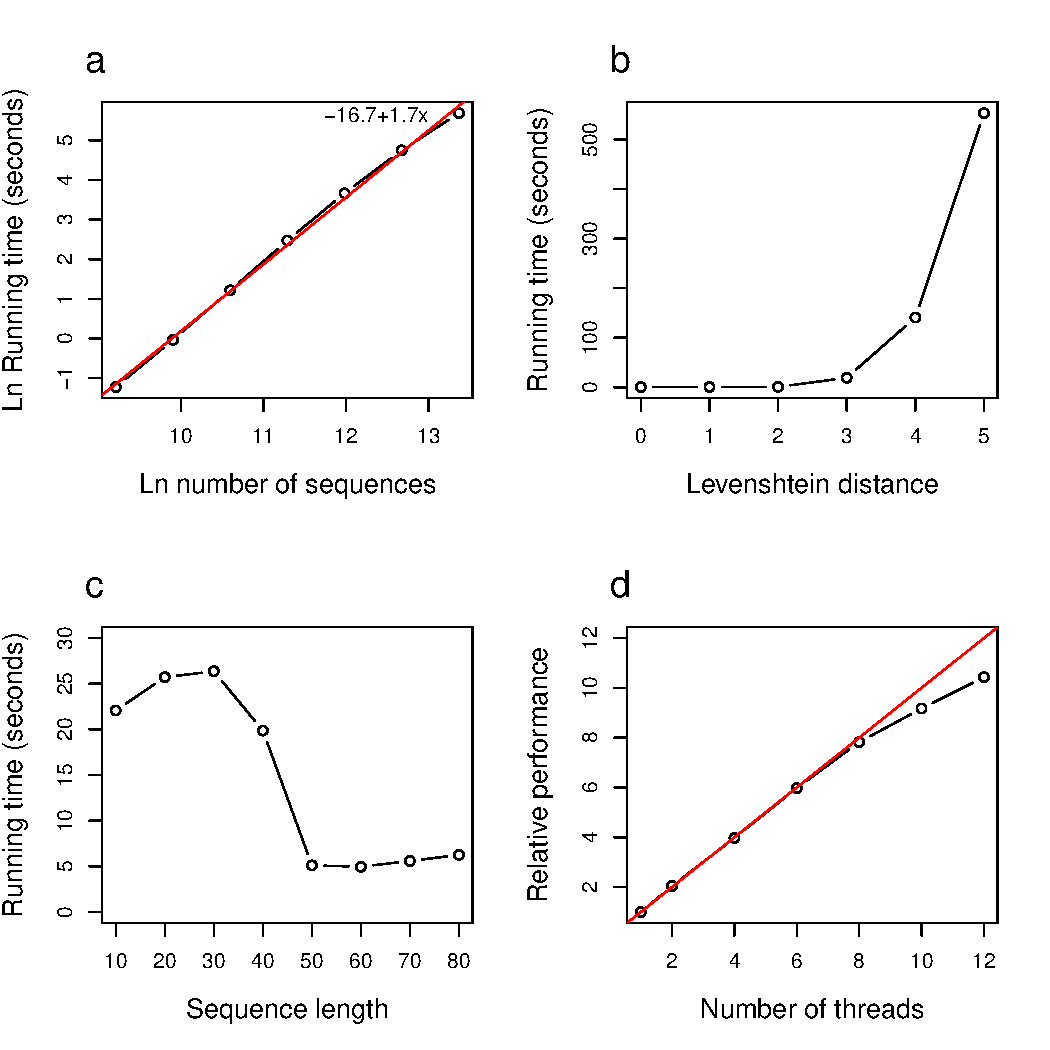
\includegraphics[scale=0.47]{scalability.pdf}}
\caption{Scalability. \textbf{a} Logarithm of the running time versus the
logarithm of the number of sequences to be clustered. \textbf{b}
Running time as a function of the clustering distance. \textbf{c}
Running time versus length of the input sequences. \textbf{d} Relative
performance increase for different number of parallel threads. 
}\label{fig:perf}
\end{figure}

\subsection{Benchmark}
\label{section:benchmark}
We benchmarked starcode against the sequence clustering algorithms
slidesort \citep{pmid21148542}, seed \citep{pmid21810899},
rainbow \citep{pmid22942077} and cd-hit \citep{pmid23060610}. Even though
slidesort is an all-pairs search algorithm, it was included in the
benchmark because sequence comparison is the most computationally
intensive step of the sequence clustering problem. Rainbow runs
exclusively on paired-end reads, whereas the other tools run on single
reads, for this reason all the tools could not be run on the same
dataset.

%% Synthetic data %%
The performance of sequence clustering algorithms can be sensitive
to the size of the clusters in the dataset, which in many applications
is not known \textit{a priori}. We therefore set up a benchmark on
artificial datasets to test the accuracy and the scaling of the
tools on a known cluster structure. We generated 4 datasets of 1 million
50-mers arranged in 1 to 1,000 clusters. Each cluster consisted
of 100 repeats of the same centroid sequence, plus satellites
derived from the centroid by incorporating 3 errors including at
most 1 indel. The number of satellites per cluster ranged from
999900 to 900. Rainbow was not tested on this benchmark because
the generated data are single reads. In addition, evaluating the
exactness of slidesort was problematic because the number of
3-matches in each dataset is not known (pairs of satellites
in the same cluster may be 3-matches or not). For this reason
we only compared the number of pairs found by starcode with
the number of pairs found by slidesort. The outcome of the test
is summarized in Figure \ref{fig:benchmark}.

\begin{figure}[!tpb]
\centerline{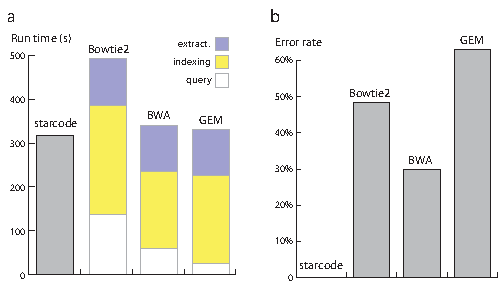
\includegraphics[scale=0.47]{benchmark.pdf}}
\caption{Benchmark results on artificial datasets of known cluster
structure (see main text). \textbf{a} Accuracy measured by the number
of identified clusters. Starcode identifies the correct
number of clusters, while seed and cd-hit identify about 40 false
positives per true positive. The red line is the first bisector and
indicates perfect results. \textbf{b} Accuracy measured by the
number of identified pairs. Slidesort identifies 5-10\% less pairs
than starcode. The red line indicates a ratio of 1. \textbf{c}
Running time of the different tools. As the size of the clusters
the running time of starcode increases but remains competitive.
\textbf{d} Memory usage of the different tools. The memory usage
of starcode decreases as the size of the cluster increases.}
\label{fig:benchmark}
\end{figure}

While starcode achieves perfect clustering on all 4 datasets, the
clustering achieved by seed and cd-hit is incomplete. Both tools
identify approximately 40 false clusters per true cluster on all
the datasets (Figure \ref{fig:benchmark}a). We also observed that
slidesort found 5-10\% less 3-matches than starcode on all the
datasets (Figure \ref{fig:benchmark}b). We were surprised by 
this result because slidesort is claimed to be an exact algorithm.
However, this was clearly not the case when we ran additional tests
on smaller datasets where naive pairwise comparisons are feasible
(more information is available on the starcode repository, see
http://github.com/gui11aume/starcode/tree/master/misc).

The running time of the different tools as a function of the size
of the clusters is shown on Figure \ref{fig:benchmark}c. The running
time of slidesort and starcode show linear and sub-linear trends,
respectively. Seed and cd-hit run approximately in constant time
regardless of the cluster size. In spite of this result, the
performance of starcode remains competitive, even for clusters of 1
million sequences. The memory usage is shown in Figure
\ref{fig:benchmark}c. The smallest memory footprint is achieved by
slidesort and cd-hit, with a maximum difference of an order of
magnitude with respect to the other tools. Note that the comparison with
slidesort is not completely fair since it does not hold in memory the
full graph necessary for clustering. The memory usage of starcode is
the highest for clusters of size 1000, but it decreases and becomes
lower than the memory usage of seed as the size of the cluster increases.
In conclusion, starcode was the only tool to achieve perfect precision
on these datasets at a price of increased memory
footprint. Considering the exactness of the output, starcode maintains
a competitive performance in terms of running time.


%% Biological datasets %%
The performance on artificial data is not always in agreement with
the performance on experimental datasets. Typical experiments present
additional difficulties. For instance,
the sizes of the clusters may be uneven and the reads may contain near
constant regions that usually degrade the performance of filter-based
algorithms. We benchmarked sequence clustering algorithms on the
problem of clustering TRIP barcodes \citep{pmid23953119}. Briefly, the
principle of TRIP (Thousands of Reporters Integrated in Parallel) is
to tag reporter transcripts with random barcodes and measure the
abundance of barcodes in the RNA as a proxy for gene expression. There
is no reference to match aberrant barcodes against, because the
tagging sequences are unknown.

The basic properties of the datasets used for benchmarking are
summarized in Table~\ref{tab:biobench_properties}. Dataset 1
(SRR950457) has been pre-processed to extract the barcode and remove
the constant part of the reads. Only barcodes between 15 and 17
nucleotides were included in the file. Dataset 2 (PRJEB7686) consists
of raw Illumina single reads. These datasets differ by the read size,
the total read count and by the empirical cluster sizes. According to
the output of starcode, the largest clusters of dataset 1 contain
approximately 70,000 sequences, whereas dataset 2 contains 4 clusters
with more than 1 million sequences. Dataset 3 (SRR950477) has been
included to benchmark starcode against rainbow in paired-end
clustering mode.
\begin{table}[h]
\centering
\caption{Summary of the biological datasets used for benchmarking.
All the datasets are Illumina reads.}
\begin{tabular}{l|c c c}
    \textit{dataset}   & \textit{read count} &
    \textit{read length} & \textit{type} \\ \hline
    SRR950457 & 6,542,309    & $16\pm 1$ & single     \\
    PRJEB7686 & 127,675,537  & 50        & single     \\
    SRR950477 & 2,460,226    & 100+100     & paired-end \\
\end{tabular}
\label{tab:biobench_properties}
\end{table}

The running times of starcode, seed, slidesort, rainbow and cd-hit
are summarized in Table~\ref{tab:biobench_runtime}. We accommodated the
distance threshold for the first dataset to compensate for the reduced
sequence length. Both starcode and slidesort were executed with
the option `\texttt{-d 2}' and the identity for cd-hit was set to
`\texttt{-c 0.85}'. We
were not able to run seed on dataset 1 due to limitations on the
minimum sequence length. Starcode was significantly faster than the other
tools on all the datasets. Seed and cd-hit came in second position
with a running time approximately 35 and 20 times greater on datasets
1 and 2, respectively. Rainbow was nearly an order of magnitude slower
in the job of clustering paired-end reads. We did not record the exact
running times past 10 days since this is several orders of magnitude
higher than the running time of starcode.

\begin{table}[h]
\centering
\caption{Running time (in seconds) of the software on three biological
datasets. Exact running time was not recordeed past 10 days.
A dash indicates that the software cannot be used for this dataset.}
\begin{tabular}{l|c c c}
    \textit{software}   & \textit{SRR950457} &
      \textit{PRJEB7686} & \textit{SRR950477} \\ \hline
    starcode   & 5           & 2,898       & 44    \\
    seed       & -           & 60,374      & -     \\
    slidesort   & 4,055       & $>$ 10 days & -     \\
    rainbow    & -           & -           & 306   \\
    cd-hit-est & 170         & 512,591     & -     \\
\end{tabular}
\label{tab:biobench_runtime}
\end{table}

The memory footprint of the different tools on the same datasets is
shown in Table~\ref{tab:biobench_memory}. The values represent the
peak memory usage throughout the run on the datasets described
above. On short reads (dataset 1), starcode outperforms the other
tools taking advantage of the trie compaction. On dataset 3, starcode
had a significantly larger memory usage than rainbow. Starcode and
cd-hit used similar amount of memory on dataset 2. Both needed twice
as much memory as slidesort, which has the advantage of not storing
the complete graph during the all-pair comparison.

\begin{table}[h]
\centering
\caption{Memory usage (in GB).}
\begin{tabular}{l|c c c}
    \textit{software}   & \textit{SRR950457} &
      \textit{PRJEB7686} & \textit{SRR950477} \\ \hline
    starcode   & 0.65 & 30.9 & 5.2 \\
    seed       & -    & 53.9 & -   \\
    slidesort   & 1.30 & 13.9 & -   \\
    rainbow    & -    & -    & 0.5 \\
    cd-hit-est & 0.80 & 28.5 & -   \\
\end{tabular}
\label{tab:biobench_memory}
\end{table}


\subsection{Identifying enriched sequence motifs}
\label{section:motifs}
As a sequence clustering algorithm, starcode can also be used for
other applications, such as the identification of enriched motifs.
Sequence motifs are thought to play an important role in DNA metabolism.
Key regulators, such as transcription factors, nucleosomes and non
coding RNAs have sequence preferences targeting them to the sites where
they act. Identifying those sequences is a way to pinpoint the
regulators and the mechanisms they are involved in. However, the
sequence motifs are not strictly identical at different sites, hence
they are better identified by inexact matching. This problem becomes
computationally difficult for long motifs (above 12-13 nucleotides)
because of the combinatorial scaling.

%But as motifs become longer, the
%problem of identifying abundant inexact matches becomes similar to
%barcode clustering. We reasoned that starcode could also be used for
%the task of identifying biologically meaningful sequence motifs.

We set up a test based on the meningitis-causing agent
\textit{Neisseria meningitidis}. The genome of this bacterium is
interspersed with a frequent 12 bp sequence known as DNA uptake
sequence \citep{pmid10673000}. We extracted the 12-mers from both
orientations of �the 2.19 Mb genome, yielding 4.39 million 12-mers,
consisting of 2.77 million unique sequences. Clustering the 12-mers
with starcode within a Levenshtein distance of 2,
%took less than 45
%seconds with 12 threads. We identified the known DNA uptake sequence
we identified the known DNA uptake sequence
of \textit{Neisseria meningitidis} (ATGCCGTCTGAA) as the most abundant
12-mer, with 1466 exact and 2096 inexact hits. This result testifies
to the fact that starcode can be used to identify biologically
relevant motifs in bacterial genomes.

To test starcode on another application, we used the RNA-protein
interaction data produced by RNAcompete \citep{pmid19561594}. The
mammalian splicing factor SRSF1 is known to bind RNA GA-rich motifs,
but there is some disagreement about the motif that it recognizes
\citep{pmid23562324}. For each replicate of the human SRSF1 in the
RNAcompete dataset, we replaced the microarray signals by their rank
and extracted the 10-mers from the microarray probes. The 10-mers were
given a score equal to the rank of the probe they belong, and enriched
motifs were found using the sphere clustering of starcode with maximum
Levenshtein distance 2. The score of the most enriched 10-mer is thus
the sum of the ranks of all 10-mers within this distance.
%Clustering
%the 6.3 million extracted 10-mers with 12 threads took about 20 seconds
%for each replicate.  The most enriched 10-mers were AGGACACGGA,
Among the 6 replicates, the most enriched 10-mers were AGGACACGGA,
AGGACACGGA, AGGACGGAGG, AGGACGGAGG, AGGACACGGA and AGGATACAGG. Except
for the last replicate, the motifs consist of AGGAC and GGA, with a
spacer of variable length. This suggests that the binding of SRSF1 to
RNA may involve a spacer sequence, which would explain the disagreement
between the motifs derived from 6-mers or 7-mers.

\section{Discussion and conclusion}
Starcode is a solid algorithm for sequence clustering based on
all-pairs matching. It achieves high precision, and on experimental
datasets it can be faster than popular heuristics. By design,
starcode is tailored to process high throughput sequencing data
on multi-core platforms with sufficient amount of memory. Due to its
superior precision and faster running time, it fills a gap among
available software, by allowing to take full advantage of middle
to high end hardware.

It is somehwat surprising that starcode is significantly faster
than competing tools on experimental datasets, whereas seed and cd-hit
are faster on artificial datasets. Starcode was developed ground up
from TRIP experimental datasets and the poucet search was selected for
giving the best empirical results. We speculate that the trie structure
benefits from the entropy deficit that is typically observed in
experimental data versus pseudorandom reads. 

The speed and precision of starcode also makes it useful for other
clustering tasks, such as identifying enriched motifs in microbial
genomes and in experimental data. Here we have given two examples of such
applications. In the first, we recover a known enriched 12-mer in the
genome of \textit{Neisseria meningitidis}. In the second, we recover
the motif of the human RNA binding protein SRSF1 and notice that it
seems to consist of two halves separated by a linker. This hypothesis
is consistent with the fact that SRSF1 binds RNA through two
consecutive RNA Recognition Motifs (RRM) that are known to bind
3-4 nucleotides in a row\citep{pmid23253355}. The Levenshtein distance,
which incorporates insertions and deletions is more likely to capture
bi-partite binding motifs than position weight matrix representations.
The use of a clustering method to tackle this problem is unusual, but it
illustrates the potential advantages of distance-based approaches.

One of the reasons why starcode appears to be faster than alternative
tools is that it is designed to cluster relatively similar sequences.
When clustering related but
divergent sequences, the Levenshtein distance will have to be increased,
leading to exponentially longer running times (Figure \ref{fig:perf}b).
However, for the imporant practical case of correcting errors introduced
by sequencing, starcode illustrates that there is still room for
developing algorithms that are both faster and more accurate than
the current state of the art.


%%%%%%%%%%%%%%%%%%%%%%%%%%%%%%%%%%%%%%%%%%%%%%%%%%%%%%%%%%%%%%%%%%%%%%%%%%%%%%%%%%%%%
%
%     please remove the " % " symbol from \centerline{\includegraphics{fig01.eps}}
%     as it may ignore the figures.
%
%%%%%%%%%%%%%%%%%%%%%%%%%%%%%%%%%%%%%%%%%%%%%%%%%%%%%%%%%%%%%%%%%%%%%%%%%%%%%%%%%%%%%%


\section*{Acknowledgement}
We would like to thank Maria Chatzou for her precious feedback on the
preliminary version of this manuscript and Heng-Chang Chen for
performing the \textit{Drosophila} TRIP experiments.

\paragraph{Funding\textcolon}
This research was funded by the Government of Catalonia (Dept. of
Economy and Knowledge) and the Spanish
Ministry of Economy and Competitiveness (Centro de Excelencia Severo Ochoa
2013-2017' (SEV-2012-0208). P.C. fellowship is partly financed by the
Spanish Ministry of Economy and Competitiveness (State Training Subprogram:
predoctoral fellowships for the training of PhD students (FPI) 2013).

\bibliographystyle{natbib}
%\bibliographystyle{achemnat}
%\bibliographystyle{plainnat}
%\bibliographystyle{abbrv}
%\bibliographystyle{bioinformatics}
%
%\bibliographystyle{plain}
%
\bibliography{document}


%\begin{thebibliography}{}
%\end{thebibliography}
\end{document}
